\documentclass[tikz,border=8pt]{standalone}
% Shared look for every TikZ diagram. Load with \input{../../tools/tikz-style.tex}
\usepackage[T1]{fontenc}
\usepackage{lmodern}
\renewcommand{\sfdefault}{lmr}  % diagrams use the same serif as the text
\usetikzlibrary{arrows.meta, positioning, shapes.geometric, calc, fit, backgrounds}
\definecolor{cblue}{HTML}{4C78A8}
\definecolor{corange}{HTML}{F58518}
\definecolor{cgreen}{HTML}{54A24B}
\definecolor{cred}{HTML}{E45756}
\definecolor{cpurple}{HTML}{B279A2}
\definecolor{cgrey}{HTML}{6B6B6B}
\tikzset{
  every picture/.style={font=\sffamily, line width=1.2pt},
  box/.style={draw=#1, fill=#1!12, rounded corners=4pt, align=center, inner sep=7pt, minimum height=1.1cm},
  box/.default=cgrey,
  arrow/.style={-{Stealth[length=3mm]}, draw=cgrey, line width=1.4pt},
  title/.style={font=\sffamily\bfseries\Large},
  note/.style={font=\sffamily\small, text=cgrey, align=center},
}
\AtBeginDocument{\hyphenpenalty=10000 \exhyphenpenalty=10000}

\usetikzlibrary{matrix}
\begin{document}
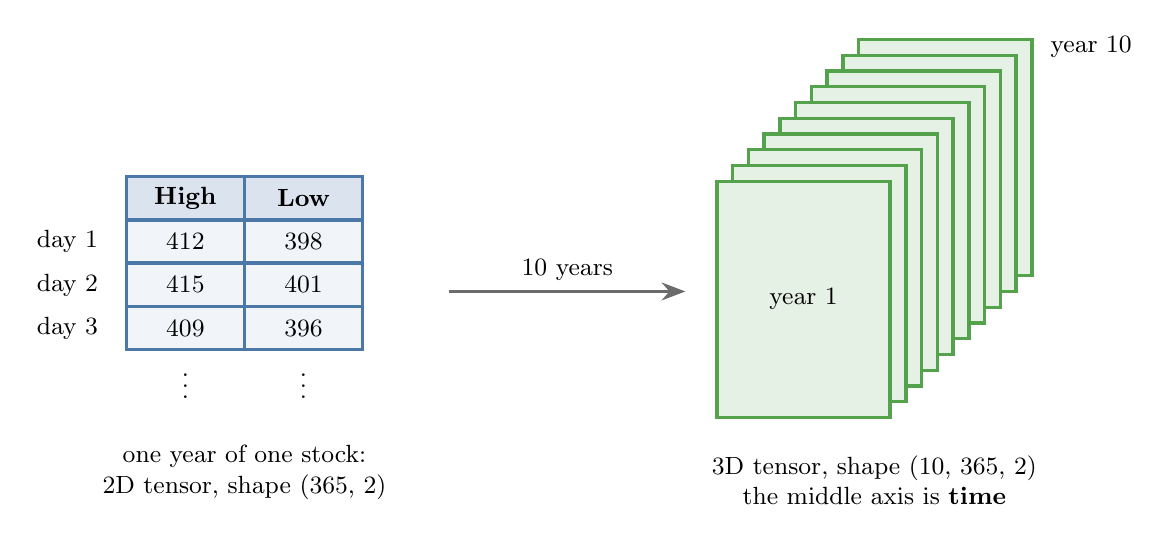
\begin{tikzpicture}
  \matrix (m) [matrix of nodes, column sep=-\pgflinewidth, row sep=-\pgflinewidth,
      nodes={minimum width=1.5cm, minimum height=0.55cm, anchor=center, draw=cblue, fill=cblue!8, font=\small},
      row 1/.style={nodes={font=\small\bfseries, fill=cblue!20}}]
  { High & Low \\ 412 & 398 \\ 415 & 401 \\ 409 & 396 \\ |[draw=none,fill=none]|\vdots & |[draw=none,fill=none]|\vdots \\ };
  \node[left=0.2cm of m-2-1, font=\small] {day 1}; \node[left=0.2cm of m-3-1, font=\small] {day 2}; \node[left=0.2cm of m-4-1, font=\small] {day 3};
  \node[below=0.2cm of m, align=center, font=\small] {one year of one stock:\\2D tensor, shape (365, 2)};
  % 10 years stacked
  \foreach \k in {9,...,0} \filldraw[draw=cgreen, fill=cgreen!15] (6+\k*0.2,-1.6+\k*0.2) rectangle ++(2.2,3.0);
  \node[font=\small, align=center] at (7.1,-0.1) {year 1};
  \node[font=\small, anchor=west] at (10.1,3.1) {year 10};
  \draw[arrow] (2.6,0) -- (5.6,0) node[midway, above, font=\small] {10 years};
  \node[align=center, font=\small] at (8.0,-2.4) {3D tensor, shape (10, 365, 2)\\the middle axis is \textbf{time}};
\end{tikzpicture}
\end{document}
